%
% interpolation.tex
%
% (c) 2024 Prof Dr Andreas Müller
%
\begin{figure}
\centering
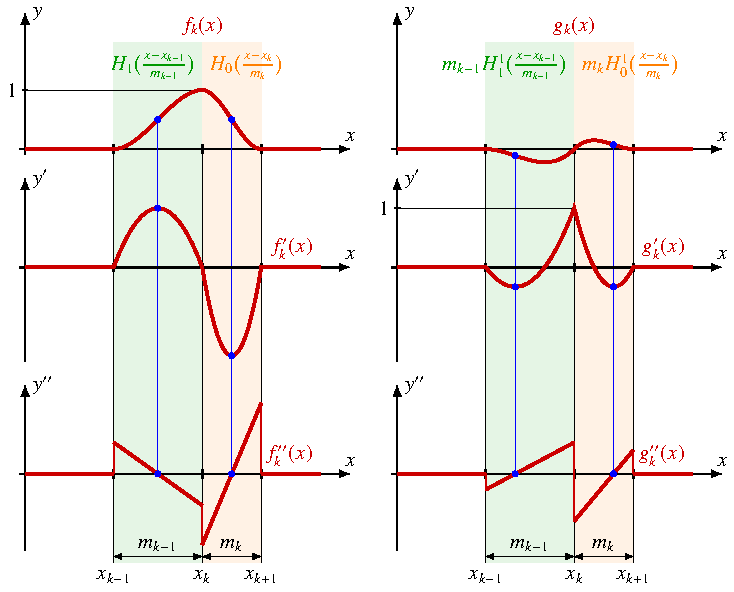
\includegraphics{chapters/030-nichtdiff/images/interpolation.pdf}
\caption{Basisfunktionen für die Spline-Interpolationsfunktion.
Die Spline-Interpolationsfunktion $y(x)$ ist Linearkombination der
Funktion $f_k(x)$, die nur an der Stützstellen $x_k$ den von Null
verschiedenen Wert $1$ und an allen Stützstellen verschwindende
Ableitung haben, und den Funktionen $g_k(x)$, deren Funktionswerte
an den Stützstellen verschwinden und deren Ableitungen nur an der
Stützstelle $x_k$ den von 0 verschiedenen Wert $1$ haben.
Die zweiten Ableitungen von $f_k(x)$ und $g_k(x)$ sind nicht
mehr stetig.
\label{buch:nichtdiff:splines:fig:interpolation}}
\end{figure}
